% !TEX TS-program = pdflatex
% !TEX encoding = UTF-8 Unicode


% This file is a template using the "beamer" package to create slides for a talk or presentation
% - Giving a talk on some subject.
% - The talk is between 15min and 45min long.
% - Style is ornate.


% MODIFIED by Jonathan Kew, 2008-07-06
% The header comments and encoding in this file were modified for inclusion with TeXworks.
% The content is otherwise unchanged from the original distributed with the beamer package.


\documentclass{beamer}




% Copyright 2004 by Till Tantau <tantau@users.sourceforge.net>.
%
% In principle, this file can be redistributed and/or modified under
% the terms of the GNU Public License, version 2.
%
% However, this file is supposed to be a template to be modified
% for your own needs. For this reason, if you use this file as a
% template and not specifically distribute it as part of a another
% package/program, I grant the extra permission to freely copy and
% modify this file as you see fit and even to delete this copyright
% notice.




\definecolor{colourname}{rgb}{.125,.5,.25}
\usecolortheme[named=colourname]{structure}
\usefonttheme{serif}
\usefonttheme{structureitalicserif}
\mode<presentation>
{
\usetheme{Warsaw}
% or ...


\setbeamercovered{transparent}
% or whatever (possibly just delete it)
}


\usepackage[english]{babel}
% or whatever


\usepackage[utf8]{inputenc}
% or whatever


\usepackage{palatino}
\usepackage[T1]{fontenc}
% Or whatever. Note that the encoding and the font should match. If T1
% does not look nice, try deleting the line with the fontenc.


\usepackage{graphicx}

% Our macros
\newcommand{\hep}{home equity position}
\newcommand{\Hep}{Home equity position}
\newcommand{\HEP}{Home Equity Position}

% Slideshow Metadata
%%%%%%%%%%%%%%%%%%%%%%%%%%%%%%
\title[Proposal] % (optional, use only with long paper titles)
{Proposal:}


\subtitle
{Preliminary Investigations of \HEP\ Markets } % (optional)


\author[Searle-White, Baron] % (optional, use only with lots of authors)
{E.~Searle-White\inst{1} \and D.~Baron\inst{2}}
% - Use the \inst{?} command only if the authors have different
% affiliation.


\institute % (optional, but mostly needed)
{
\inst{1}%
Mills College
\and
\inst{2}%
Western Washington University
}
% - Use the \inst command only if there are several affiliations.
% - Keep it simple, no one is interested in your street address.


\date[EUR Introduction] % (optional)
{September 24/ BSM Research Project Introductory Talks}


\subject{Financial Mathematics}
% This is only inserted into the PDF information catalog. Can be left
% out.






% If you have a file called "university-logo-filename.xxx", where xxx
% is a graphic format that can be processed by latex or pdflatex,
% resp., then you can add a logo as follows:


% \pgfdeclareimage[height=0.5cm]{university-logo}{university-logo-filename}
% \logo{\pgfuseimage{university-logo}}






% Delete this, if you do not want the table of contents to pop up at
% the beginning of each subsection:
\AtBeginSection[]
{
\begin{frame}<beamer>{Outline}
\tableofcontents[currentsection]
\end{frame}
}

\AtBeginSubsection[]
{
\begin{frame}<beamer>{Outline}
\tableofcontents[currentsection,currentsubsection]
\end{frame}
}

% If you wish to uncover everything in a step-wise fashion, uncomment
% the following command:


%\beamerdefaultoverlayspecification{<+->}






\usepackage{parskip}




\begin{document}


\begin{frame}
\titlepage
\end{frame}


\begin{frame}{Outline}
\tableofcontents
% You might wish to add the option [pausesections]
\end{frame}




% Since this a solution template for a generic talk, very little can
% be said about how it should be structured. However, the talk length
% of between 15min and 45min and the theme suggest that you stick to
% the following rules:


% - Exactly two or three sections (other than the summary).
% - At *most* three subsections per section.
% - Talk about 30s to 2min per frame. So there should be between about
% 15 and 30 frames, all told.
%
% - A conference audience is likely to know very little of what you
% are going to talk about. So *simplify*!
% - In a 20min talk, getting the main ideas across is hard
% enough. Leave out details, even if it means being less precise than
% you think necessary.
% - If you omit details that are vital to the proof/implementation,
% just say so once. Everybody will be happy with that.


\section{Introduction}


\begin{frame}{Introduction}
We can use mathematics to model and understand the behavior of financial systems.

With respect to existing markets, such as stock exchanges and housing markets, these applications are well understood. 

\begin{itemize}
\item
Our project: define and study a new type of financial instrument.
\begin{itemize}
\item 
How useful are the existing tools and methods of financial mathematics in this context?
 \item 
What new methods need to be developed?
\end{itemize}
\end{itemize}
\end{frame}


\begin{frame}{The Home Equity Position and the Market}{}
\textbf{Definition:} A \emph{home equity position} is a claim on a fixed percentage of the equity in a particular owner-occupied residence.\bigskip

A homeowner $A$ offers a new \hep\ on the Primary Market for a fixed asking price $P$. Investors then bid down the percentage claim value $C$ of the position until a bid is accepted and the position is sold for that fixed price.

\end{frame}
\begin{frame}{Home Equity Position Exchange}
\Hep\ trading:


The \hep\ can then be traded in the manner of a stock on the Secondary Market. Note: multiple investors can co-own a single \hep.

We will often simply refer to this secondary exchange as \emph{"the market"}.
\end{frame}








\section{Existing Methodologies}

\subsection{Securities Exchanges}
\begin{frame}{Securities Exchanges}{Characteristics and Standard Approaches}
% - A title should summarize the slide in an understandable fashion
% for anyone how does not follow everything on the slide itself.
There is a wealth of literature on the subject of equity markets. Several factors involved in traditional equity exchanges will be relevant to this new market, including:
\begin{itemize}
\item
Supply/Demand
\item
Speculation
\item
Investor Behavior
\item
Stochastic Processes
\end{itemize}
\end{frame}

\subsection{Housing Markets}
\begin{frame}{Housing Markets}{Characteristics and Standard Approaches}
Real Estate markets are influenced by many of the same factors as other equity markets, but they have a few unique characteristics:
\pause
\begin{itemize}
\item
Durability of the Commodity
\pause
\item
High Transaction Costs
\pause
\item
Heterogeneity
\pause
\item
Dual Use of the Commodity
\end{itemize}

\end{frame}


\section{Unique Considerations}

\begin{frame}{Home-Equity Exchange}
\begin{itemize}
\item
In a market with similarities to both of these, which factors will still be important? Which evaluation techniques will still be relevant?
\item
In short, what existing ideas apply % Or "existing theory"?
 to this new market and what new approaches does it demand? 
\end{itemize} 
\end{frame}


\begin{frame}{Key Differences}
Some new characteristics of a Home-Equity market:
\pause
\begin{itemize}
\item
Individuality/heterogeneity
\pause
\item
Importance of local economies
\pause
\item
Dependence (Investor/Homeowner)
\end{itemize}

\end{frame}




\begin{frame}{Further Differences}
\begin{itemize}
\item
Risk/Return
\item
Liquidity
\item
Tax Structure (1031 Exchange)
\item
Pricing Structure
\item
Portfolio Diversification
\end{itemize}
\end{frame}

\section{Plan of Action}
\begin{frame}{Questions To Be Explored}
\pause
\begin{itemize}
\item
What behaviors might be typical in this new market?
\pause
\item
What kinds of events could trigger a crash in this market?
\pause
\item
Are the standard tools for evaluation of traditional markets still useful in this situation?
\pause
\item
In addition, how might a market like this grow from the very beginning, as it has not yet been established? How do dynamics change with additions of new cities, new types of investors?
\end{itemize}
\end{frame}

\begin{frame}{First Steps}
At the beginning of the semester, each week Dan and Emily will review topics in
\begin{itemize}
\item
Stochastic Calculus
\begin{itemize}
\item
Brownian Motion
\item
Random Walks
\item
Markov Chains
\end{itemize}
\item
Quantitative Finance
\begin{itemize}
\item
Portfolio Theory
\item
Univariate/Multivariate Risk Assessment.
\end{itemize}
\end{itemize}

\end{frame}

\begin{frame}{Methods and Models}

In weekly meetings with Rozi we will discuss the aforementioned topics and build simple computer models to understand market dynamics.

Concurrently, we will begin to apply these concepts and construct more complex models of the new \hep\ market.
\end{frame}

\begin{frame}
%\begin{center} 
Thank you for your time and attention.

We appreciate the opportunity to pursue this research at BSM. We are grateful in particular to our project advisors Dezs\H o and Rozi Miklos. 

Also, a special thank you to Agnes for listening to all of Emily's emails.

 
 %  \end{center}
\end{frame}

\begin{frame}{Questions?}
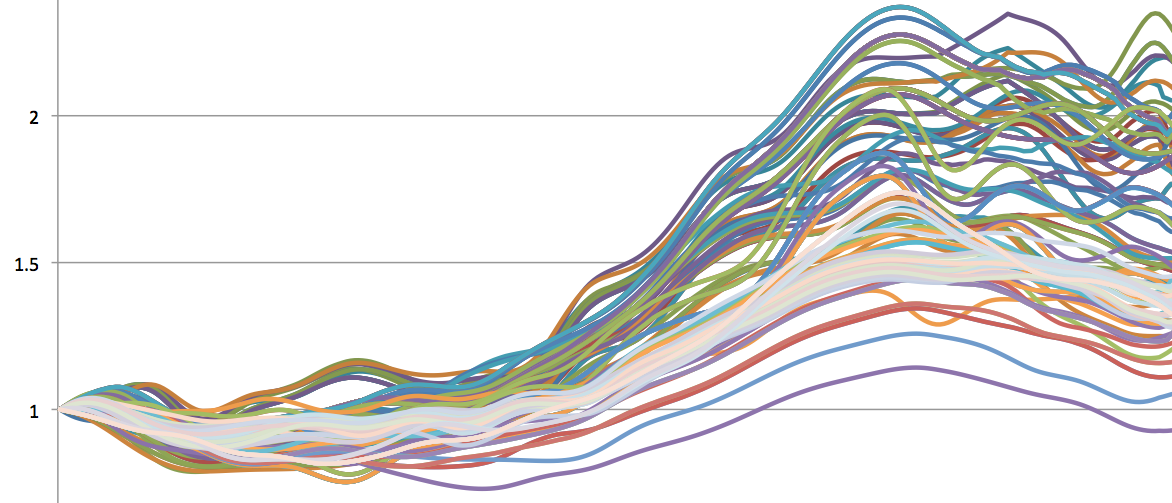
\includegraphics[scale = .35]{yay.png}

\end{frame}


\end{document}






